\PassOptionsToPackage{unicode=true}{hyperref} % options for packages loaded elsewhere
\PassOptionsToPackage{hyphens}{url}
%
\documentclass[]{article}
\usepackage{lmodern}
\usepackage{amssymb,amsmath}
\usepackage{ifxetex,ifluatex}
\usepackage{fixltx2e} % provides \textsubscript
\ifnum 0\ifxetex 1\fi\ifluatex 1\fi=0 % if pdftex
  \usepackage[T1]{fontenc}
  \usepackage[utf8]{inputenc}
  \usepackage{textcomp} % provides euro and other symbols
\else % if luatex or xelatex
  \usepackage{unicode-math}
  \defaultfontfeatures{Ligatures=TeX,Scale=MatchLowercase}
\fi
% use upquote if available, for straight quotes in verbatim environments
\IfFileExists{upquote.sty}{\usepackage{upquote}}{}
% use microtype if available
\IfFileExists{microtype.sty}{%
\usepackage[]{microtype}
\UseMicrotypeSet[protrusion]{basicmath} % disable protrusion for tt fonts
}{}
\IfFileExists{parskip.sty}{%
\usepackage{parskip}
}{% else
\setlength{\parindent}{0pt}
\setlength{\parskip}{6pt plus 2pt minus 1pt}
}
\usepackage{hyperref}
\hypersetup{
            pdftitle={Comparativo de Modelos},
            pdfauthor={Sebastian Jaremczuk},
            pdfborder={0 0 0},
            breaklinks=true}
\urlstyle{same}  % don't use monospace font for urls
\usepackage[margin=1in]{geometry}
\usepackage{listings}
\newcommand{\passthrough}[1]{#1}
\usepackage{graphicx,grffile}
\makeatletter
\def\maxwidth{\ifdim\Gin@nat@width>\linewidth\linewidth\else\Gin@nat@width\fi}
\def\maxheight{\ifdim\Gin@nat@height>\textheight\textheight\else\Gin@nat@height\fi}
\makeatother
% Scale images if necessary, so that they will not overflow the page
% margins by default, and it is still possible to overwrite the defaults
% using explicit options in \includegraphics[width, height, ...]{}
\setkeys{Gin}{width=\maxwidth,height=\maxheight,keepaspectratio}
\setlength{\emergencystretch}{3em}  % prevent overfull lines
\providecommand{\tightlist}{%
  \setlength{\itemsep}{0pt}\setlength{\parskip}{0pt}}
\setcounter{secnumdepth}{0}
% Redefines (sub)paragraphs to behave more like sections
\ifx\paragraph\undefined\else
\let\oldparagraph\paragraph
\renewcommand{\paragraph}[1]{\oldparagraph{#1}\mbox{}}
\fi
\ifx\subparagraph\undefined\else
\let\oldsubparagraph\subparagraph
\renewcommand{\subparagraph}[1]{\oldsubparagraph{#1}\mbox{}}
\fi

% set default figure placement to htbp
\makeatletter
\def\fps@figure{htbp}
\makeatother

\usepackage{booktabs}
\usepackage{longtable}
\usepackage{array}
\usepackage{multirow}
\usepackage{wrapfig}
\usepackage{float}
\usepackage{colortbl}
\usepackage{pdflscape}
\usepackage{tabu}
\usepackage{threeparttable}
\usepackage{threeparttablex}
\usepackage[normalem]{ulem}
\usepackage{makecell}
\usepackage{xcolor}

\title{Comparativo de Modelos}
\author{Sebastian Jaremczuk}
\date{2020-04-17}

\begin{document}
\maketitle

\hypertarget{carga-de-datos}{%
\subsubsection{carga de datos}\label{carga-de-datos}}

\hypertarget{comparar-modelos}{%
\section{COMPARAR MODELOS}\label{comparar-modelos}}

Una vez que se han entrenado y optimizado distintos modelos, se tiene
que identificar cuál de ellos consigue mejores resultados. La manera en
la que se van a comparar los modelos es a através de métricas de
Validación y el error en el Test.

Este análisis se realiza con todos los modelos y sus variantes usando
distintos datasets (los distintos métodos y para los que usan todos los
predictores o una selección de los mismos
\ref{otros datasets, datos reducidos por seleccion})

\hypertarget{muxe9tricas-de-valicaciuxf3n}{%
\subsection{Métricas de valicación}\label{muxe9tricas-de-valicaciuxf3n}}

Las métricas obtenidas mediante validación (cv, etc) son estimaciones de
la capacidad que tiene un modelo al predecir nuevas observaciones.

\begin{table}[!h]

\caption{\label{tab:cuadro_comparativo-modelos}Resumen comparativo de algunos los modelos empleados}
\centering
\begin{tabular}[t]{cccc}
\toprule
\rowcolor{black}  \multicolumn{1}{c}{\textcolor{white}{\textbf{object}}} & \multicolumn{1}{c}{\textcolor{white}{\textbf{Test}}} & \multicolumn{1}{c}{\textcolor{white}{\textbf{Training}}} & \multicolumn{1}{c}{\textcolor{white}{\textbf{dataset}}}\\
\midrule
\rowcolor{gray!6}  SVMradial & 0.8419898 & 0.8511438 & DataSet-Completo\\
RandomForest & 0.8405267 & 0.9103729 & DataSet-Alternativa1\\
\rowcolor{gray!6}  rf & 0.8383321 & 0.9200877 & DataSet-Completo\\
boosting & 0.8361375 & 0.8740207 & DataSet-Completo\\
\rowcolor{gray!6}  logistic & 0.8354060 & 0.8420558 & DataSet-Completo\\
\addlinespace
Reg\_logistica & 0.8339429 & 0.8345346 & DataSet-Alternativa1\\
\rowcolor{gray!6}  arbol & 0.8324799 & 0.8552178 & DataSet-Completo\\
LDA & 0.8266277 & 0.8301473 & DataSet-Completo\\
\rowcolor{gray!6}  KNN & 0.8039503 & 0.8198057 & DataSet-Completo\\
RandomForest\_5 & 0.7849305 & 0.9674083 & DataSet-Alternativa2\\
\addlinespace
\rowcolor{gray!6}  SVM\_5 & 0.7820044 & 0.7988092 & DataSet-Alternativa2\\
Reg\_logistica\_5 & 0.7717630 & 0.7768725 & DataSet-Alternativa2\\
\rowcolor{gray!6}  C50\_5 & 0.7534748 & 0.8147916 & DataSet-Alternativa2\\
GradienBoosting\_5 & 0.7520117 & 0.7963021 & DataSet-Alternativa2\\
\bottomrule
\end{tabular}
\end{table}

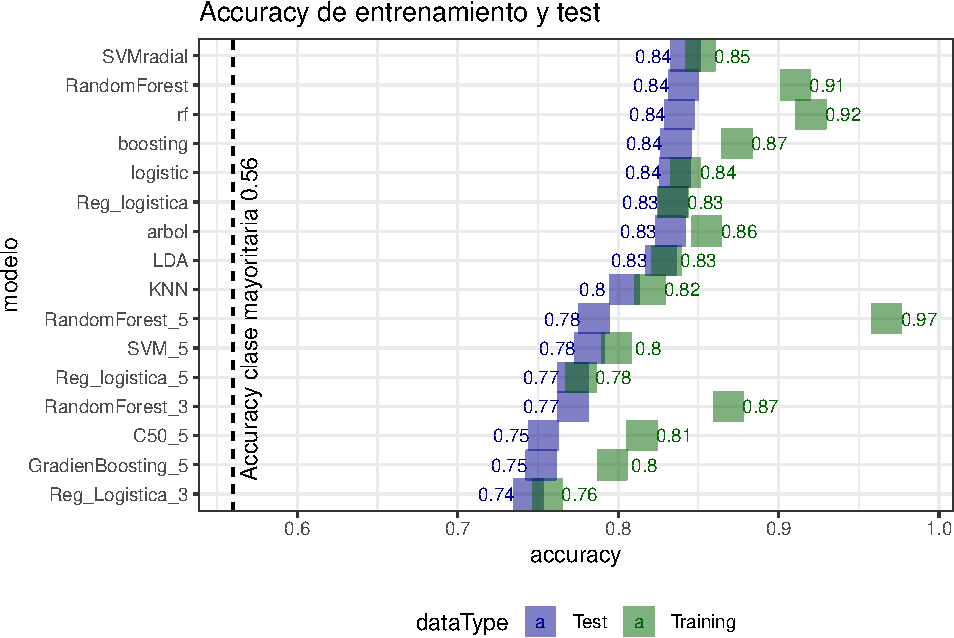
\includegraphics{Comparativo_modelos_files/figure-latex/unnamed-chunk-10-1.pdf}

Los vaores expresados en el gráfico son aquellos que una vez optimizado
los parámetros con Crossvalidation, se entrena el modelo sin particiones
utilizando todas las observaciones como train.

\hypertarget{conclusiuxf3n-de-comparacion-modelos}{%
\subsection{conclusión de comparacion
modelos}\label{conclusiuxf3n-de-comparacion-modelos}}

En los modelos que se realizan con datos completos, podemos determinar
que el mejor modelo entrenado es el que emplea el método SVM. También
resulta ser el mejor cuando se elimina la variable que mas influencia
tiene en el resultado. De los métodos explicativos se puede decir que la
regresión logistica seguido del arbol simple dan buenos resultados y no
muy alejado de las métricas de SVM.

Po rotro lado, los distintos modelos de Random Forest dan muy buenos
resultados pero hay una diferencia muy grande en comparación a los otros
métodos entre train y test, por lo que hay que ser precavido por el
riesgo de sobreajuste.

Por lo tanto, si lo importante es elegir unmodelo que tenga mejor
capacidad predictiva, con estas combinaciones de datos, la mejor opción
es un SVM. No obstante, si se prioriza la interpretabilidad del modelo
para extraer conclusiones, se podría seleccionar el modelo Regresión
Logística o arbol simple.

\end{document}
